%%%%%%%%%%%%%%%%%%%%%%%%%%%%%%%%%%%%%%%%%
% Short Sectioned Assignment LaTeX Template Version 1.0 (5/5/12)
% This template has been downloaded from: http://www.LaTeXTemplates.com
% Original author:  Frits Wenneker (http://www.howtotex.com)
% License: CC BY-NC-SA 3.0 (http://creativecommons.org/licenses/by-nc-sa/3.0/)
%%%%%%%%%%%%%%%%%%%%%%%%%%%%%%%%%%%%%%%%%

%----------------------------------------------------------------------------------------
%	PACKAGES AND OTHER DOCUMENT CONFIGURATIONS
%----------------------------------------------------------------------------------------

\documentclass[paper=a4, fontsize=11pt]{scrartcl} % A4 paper and 11pt font size

% ---- Entrada y salida de texto -----

\usepackage[T1]{fontenc} % Use 8-bit encoding that has 256 glyphs
\usepackage[utf8]{inputenc}
%\usepackage{fourier} % Use the Adobe Utopia font for the document - comment this line to return to the LaTeX default

% ---- Idioma --------

\usepackage[spanish, es-tabla]{babel} % Selecciona el español para palabras introducidas automáticamente, p.ej. "septiembre" en la fecha y especifica que se use la palabra Tabla en vez de Cuadro

% ---- Otros paquetes ----

\usepackage{amsmath,amsfonts,amsthm} % Math packages
%\usepackage{graphics,graphicx, floatrow} %para incluir imágenes y notas en las imágenes
\usepackage{graphics,graphicx, float} %para incluir imágenes y colocarlas

% Para hacer tablas comlejas
%\usepackage{multirow}
%\usepackage{threeparttable}

%\usepackage{sectsty} % Allows customizing section commands
%\allsectionsfont{\centering \normalfont\scshape} % Make all sections centered, the default font and small caps

\usepackage{fancyhdr} % Custom headers and footers
\pagestyle{fancyplain} % Makes all pages in the document conform to the custom headers and footers
\fancyhead{} % No page header - if you want one, create it in the same way as the footers below
\fancyfoot[L]{} % Empty left footer
\fancyfoot[C]{} % Empty center footer
\fancyfoot[R]{\thepage} % Page numbering for right footer
\renewcommand{\headrulewidth}{0pt} % Remove header underlines
\renewcommand{\footrulewidth}{0pt} % Remove footer underlines
\setlength{\headheight}{13.6pt} % Customize the height of the header

\numberwithin{equation}{section} % Number equations within sections (i.e. 1.1, 1.2, 2.1, 2.2 instead of 1, 2, 3, 4)
\numberwithin{figure}{section} % Number figures within sections (i.e. 1.1, 1.2, 2.1, 2.2 instead of 1, 2, 3, 4)
\numberwithin{table}{section} % Number tables within sections (i.e. 1.1, 1.2, 2.1, 2.2 instead of 1, 2, 3, 4)

\setlength\parindent{0pt} % Removes all indentation from paragraphs - comment this line for an assignment with lots of text

\newcommand{\horrule}[1]{\rule{\linewidth}{#1}} % Create horizontal rule command with 1 argument of height

\usepackage{listings}



%----------------------------------------------------------------------------------------
%	TÍTULO Y DATOS DEL ALUMNO
%----------------------------------------------------------------------------------------

\title{	
\normalfont \normalsize 
\textsc{{\bf Visi\'on por Computador (2014-2015)} \\ Grado en Ingeniería Informática \\ Universidad de Granada} \\ [25pt] % Your university, school and/or department name(s)
\horrule{0.5pt} \\[0.4cm] % Thin top horizontal rule
\huge Proyecto Final: Intelligent Scissors \\ % The assignment title
\horrule{2pt} \\[0.5cm] % Thick bottom horizontal rule
}

\author{Alberto Quesada y Javier Moreno} % Nombre y apellidos

\date{\normalsize\today} % Incluye la fecha actual

%----------------------------------------------------------------------------------------
% DOCUMENTO
%----------------------------------------------------------------------------------------

\begin{document}

\maketitle % Muestra el Título

\newpage %inserta un salto de página

\tableofcontents % para generar el índice de contenidos

\listoffigures


\newpage

 
 

\newpage

%----------------------------------------------------------------------------------------
%	Cuesti´on 1
%----------------------------------------------------------------------------------------

\section{Introducción}

En la actualidad el retoque fotográfico es una práctica cada vez más común tanto entre usuarios experimentados como amateurs. Uno de los requisitos básicos que se le suele pedir a las herramientas de edición de imagen (como Photoshop, GIMP, Pixelmator…) es la capacidad para extraer objetos de una escena. Esta tiene diferentes nombres dependiendo del software usado: Magic Wand Tool (Pixelmator), Lazo (Photoshop) o Tijeras (GIMP). \\

La delimitación de objetos manual es muy imprecisa y laboriosa. Aunque hay varias técnicas para automatizar este proceso, el problema sigue estando sin resolver por completo. La técnica propuesta para este proyecto se llama Intelligent Scissors (tijeras inteligentes) y permite extraer objetos de imágenes de forma rápida y bastante acertada.  \\

El programa desarrollado sigue la técnica descrita en el artículo mort-sigg95\footnote{http://courses.cs.washington.edu/courses/cse455/02wi/readings/mort-sigg95.pdf}, permitiendo al usuario utilizarla mediante una sencilla interfaz gráfica. No es necesario tener ningún conocimiento previo de la técnica o de ningún concepto de visión por computador.  \\

Una vez seleccionada la imagen que se desea usar y elegido el objeto que se desea extraer, se tiene que ir pulsando con el ratón sobre varios puntos que delimiten el objeto y el software buscará la el camino óptimo para segmentación entre esos puntos.

%------------------------------------------------

\section{Descripción del algoritmo}

El algoritmo está basado en programación dinámica y formulado como un problema de búsqueda en grafo. La idea básica es encontrar el camino óptimo para segmentación entre dos píxeles definidos manualmente. Este camino óptimo es creado entre los dos píxeles y sus 8 vecinos, para encontrarlo se usa una función de coste entre un pixel y uno de sus vecinos. \\

\begin{figure}[H] %con el [H] le obligamos a situar aquí la figura
\centering
\includegraphics[scale=0.4]{/Users/alberto/Desktop/1.png}  %el parámetro scale permite agrandar o achicar la imagen. En el nombre de archivo puede especificar directorios
\label{kk1}
\caption{Función de coste local} 
\end{figure}

\begin{figure}[H] %con el [H] le obligamos a situar aquí la figura
\centering
\includegraphics[scale=0.4]{/Users/alberto/Desktop/2.png}  %el parámetro scale permite agrandar o achicar la imagen. En el nombre de archivo puede especificar directorios
\label{kk1}
\caption{Cruzando por cero la laplaciana} 
\end{figure}

\begin{figure}[H] %con el [H] le obligamos a situar aquí la figura
\centering
\includegraphics[scale=0.4]{/Users/alberto/Desktop/3.png}  %el parámetro scale permite agrandar o achicar la imagen. En el nombre de archivo puede especificar directorios
\label{kk1}
\caption{Magnitud del gradiente} 
\end{figure}

\begin{figure}[H] %con el [H] le obligamos a situar aquí la figura
\centering
\includegraphics[scale=0.4]{/Users/alberto/Desktop/4.png}  %el parámetro scale permite agrandar o achicar la imagen. En el nombre de archivo puede especificar directorios
\label{kk1}
\caption{Dirección del gradiente} 
\end{figure}

\begin{figure}[H] %con el [H] le obligamos a situar aquí la figura
\centering
\includegraphics[scale=0.4]{/Users/alberto/Desktop/41.png}  %el parámetro scale permite agrandar o achicar la imagen. En el nombre de archivo puede especificar directorios
\label{kk1}
\caption{Especificación de la dirección del gradiente} 
\end{figure}

\begin{figure}[H] %con el [H] le obligamos a situar aquí la figura
\centering
\includegraphics[scale=0.4]{/Users/alberto/Desktop/5.png}  %el parámetro scale permite agrandar o achicar la imagen. En el nombre de archivo puede especificar directorios
\label{kk1}
\caption{Link bidireccional entre los pixeles p y q} 
\end{figure}

\begin{itemize}
\item fz: Cruzando por cero la laplaciana.
\item fg: Magnitud del gradiente.
\item fd: Dirección del gradiente.
\item Wz, wd, wg son valores ya definidos que fueron calculados empiricamente por los autores del algoritmo.
\end{itemize}

El algoritmo principal recibe un pixel, teniendo el grafo de costes (pudiendo estar sin calcular algunos de sus valores al estar trabajando con programación dinámica), y mediante una lista de píxeles activos ordenados mediante sus costes, se van recorriendo sus vecinos y comprobando si pertenecen al camino óptimo o no.

\section{Implementación}

Para la implementación se han usado dos clases principales Window e IntelligentScissors, la primera maneja la presentación de imágenes y la segunda gestiona el algoritmo. \\

Se ha creado una estructura llamada Pixel para gestionar el grafo de búsqueda.
\\

\begin{lstlisting}
struct Pixel
{
	bool calculated;
	double N[8];
	double cost;
	Point point;
};
\end{lstlisting}

\subsection{Clase Window}

\begin{description}
\item[Window::Window(string filePath, string windowName)] \hfill \\
	Constructor de la clase Window que recibe la imagen a mostrar y el nombre de la ventana.
\item[void Window::drawImage()]\hfill \\
	Método que dibuja la imagen en pantalla.
\item[void Window::refreshImage()] \hfill \\
	Método que actualiza la imagen en pantalla cuando ha tenido alguna modificación.
\item[void Window::touch(int event, int x, int y)]\hfill \\
	Método que controla los eventos de los clicks del ratón en la ventana de la imagen, y al seleccionar un punto lo pasa al algoritmo para construir el camino óptimo.
\item[void Window::start()]\hfill \\
	Inicio de la interfaz.

\end{description}

\subsection{Clase IntelligentScissors}

\begin{description}
\item[IntelligentScissors::IntelligentScissors(string filePath, float wZ, float wD, float wG)]\hfill \\
	Constructor de la clase IntelligentScissors que recibe la imagen a procesar. Recibe la 	imagen, la lee y la convierte a escala de grises para poder trabajar con ella.	
\item[void IntelligentScissors::initData()]\hfill \\
	Método que inicializa las estructuras de datos a usar. Elimina el ruido de la imagen mediante un filtro de Gauss, calcula la Laplaciana, los gradientes, la matriz G e inicializa las estructuras de datos necesarias para el algoritmo, entre ellas el grafo de costes.
\item[void IntelligentScissors::calculateLocalCost(Point p)]\hfill \\
	Método que construye un pixel en el punto p y calcula el coste de sus 8 vecinos. Con este método es como se va rellenando el grafo de costes, ya que es llamado cuando un pixel tiene su variable booleana de calculado a false.
\item[Pixel* IntelligentScissors::getPixel(Point p)]\hfill \\
	Devuelve un puntero a un pixel, si no está inicialado, lo inicializa. Este método es el que llamamos cuando necesitamos un pixel, o su coste entre el y uno de sus vecinos, lo que sería la función de costes del algoritmo: l(q, r).
\item[bool IntelligentScissors::checkDimensions(Point p)]\hfill \\
	Comprueba si estamos accediendo a un punto fuera de las dimensiones de la imagen.
\item[double IntelligentScissors::fZ(Point q)]\hfill \\
	Calcula el valor de fZ para el grafo de costes.
\item[double IntelligentScissors::fD(Point p, Point q)]\hfill \\
	Calcula el valor de fD para el grafo de costes.
\item[double IntelligentScissors::fG(Point q, int n)]\hfill \\
	Calcula el valor de fD para el grafo de costes.
\item[void IntelligentScissors::NormalizePoint(Point &p)]\hfill \\
	Normaliza un punto.
\item[void IntelligentScissors::NormalizeSmallValues(double &v)]\hfill \\
	Comprueba si un valor es demasiado pequeño, si es así lo iguala a 0.
\item[Point IntelligentScissors::getNeighbor(Point p, int n)]\hfill \\
	Devuelve el n vecino de un punto p.
\item[bool IntelligentScissors::isDiagonal(int n)]\hfill \\
	Comprueba si el vecino n está en la diagonal de un punto.
\item[void IntelligentScissors::setError(int error)]\hfill \\
	Devuelve un error y termina el programa.
\item[void IntelligentScissors::setPoint(int x, int y)]\hfill \\
	Define el punto siguiente en el algoritmo, lo pinta y pinta el camino óptimo que encuentra. Este es el método inicial del algoritmo.
\item[void IntelligentScissors::drawPath(Point s)]\hfill \\
	Dibuja el camino encontrado entre dos puntos.
\item[void IntelligentScissors::drawPoint(Point s)]\hfill \\
	Dibuja un punto en la imagen.
\item[void IntelligentScissors::optimalPath(Point s)]\hfill \\
	Algoritmo Live-Wire 2-D DP graph search. Calcula el camino óptimo entre dos puntos para segmentación.
\item[bool IntelligentScissors::find(multiset<Pixel*, comp> &L, Pixel* p)]\hfill \\
	Busca si un Pixel pertecene a un multiset de Pixel.
\item[const Mat& IntelligentScissors::getImage()]\hfill \\
	Devuelve la imagen.
\item[vector<Point> IntelligentScissors::getPath()]\hfill \\
	Devuelve el camino óptimo encontrado.
	
	\end{description}

Como comentario a la implementación, para mejorar la eficiencia se ha usado una estructura de datos multiset para la lista de píxeles activos ordenada por sus costes. También como mejora de eficiencia se han usado punteros a píxeles en casi todos los cálculos evitando la construcción de píxeles y pudiendo modificarlos en el grafo de costes directamente. \\

\newpage
\subsection{Algoritmo principal:}

\begin{lstlisting}
void IntelligentScissors::optimalPath(Point s)
{
	// Pointers from each pixel indicating the minimum cost path.
	P = vector<vector<Point> >(imgGray.rows, vector<Point>(
	imgGray.cols));
	
	// Boolean function indicating if q has been 
	// expanded/processed.
	vector<vector<bool> > e (imgGray.rows, vector<bool>(
	imgGray.cols, false));

	// List of active pixels sorted by total cost (initially empty).
	multiset<Pixel*, comp> L;
	
	Pixel *q, *r;
	double g_tmp;

	// Initialize active list with zero cost seed pixel.	
	getPixel(s)->cost = 0.0;
	L.insert(getPixel(s));

	while(!L.empty()) // While still points to expand.
	{
		// Remove minimum cost pixel q from active list.
		q = *L.begin(); L.erase(L.begin()); 
		e[q->point.x][q->point.y] = true; // Mark q as expanded.
		for(int n=0; n<8; n++)
		{
			Point a = getNeighbor(q->point, n);
			r = getPixel(a);			
			if(r != NULL && !e[r->point.x][r->point.y])
			{
				// Compute total cost to neighbor.
				g_tmp = q->cost + q->N[n]; 
				
				if(find(L, r))
				{
				  if(g_tmp < r->cost)
				// Remove higher cost neighbor's from list.
				    L.erase(r); 
				}
				else // if neighbor not on list.
				{
				 // assign neighbor's total cost.
				  r->cost = g_tmp; 
				 // set back pointer.
				  P[r->point.x][r->point.y] = q->point; 
				 // and place on (or return to) active list.
				  L.insert(r); 
				}
			}
		}
	}
}
\end{lstlisting}
\newpage

\section{Experimentos realizados}

Las imágenes utilizadas para valorar los resultados han sido las siguientes:

\begin{figure}[H] %con el [H] le obligamos a situar aquí la figura
\centering
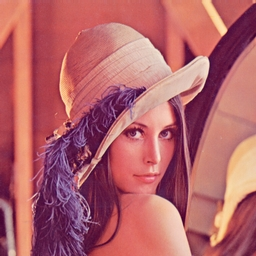
\includegraphics[scale=0.6]{/Users/alberto/Desktop/lena.jpg}  %el parámetro scale permite agrandar o achicar la imagen. En el nombre de archivo puede especificar directorios
\label{kk1}
\caption{Lena: Dificultad Media} 
\end{figure}

\begin{figure}[H] %con el [H] le obligamos a situar aquí la figura
\centering

\includegraphics[scale=0.6]{/Users/alberto/Desktop/black.jpg}  %el parámetro scale permite agrandar o achicar la imagen. En el nombre de archivo puede especificar directorios
\label{kk1}
\caption{Black: Dificultad Fácil} 
\end{figure}

\begin{figure}[H] %con el [H] le obligamos a situar aquí la figura
\centering

\includegraphics[scale=0.6]{/Users/alberto/Desktop/circle_black.jpg}  %el parámetro scale permite agrandar o achicar la imagen. En el nombre de archivo puede especificar directorios
\label{kk1}
\caption{Circle black: Dificultad Difícil} 
\end{figure}

\begin{figure}[H] %con el [H] le obligamos a situar aquí la figura
\centering
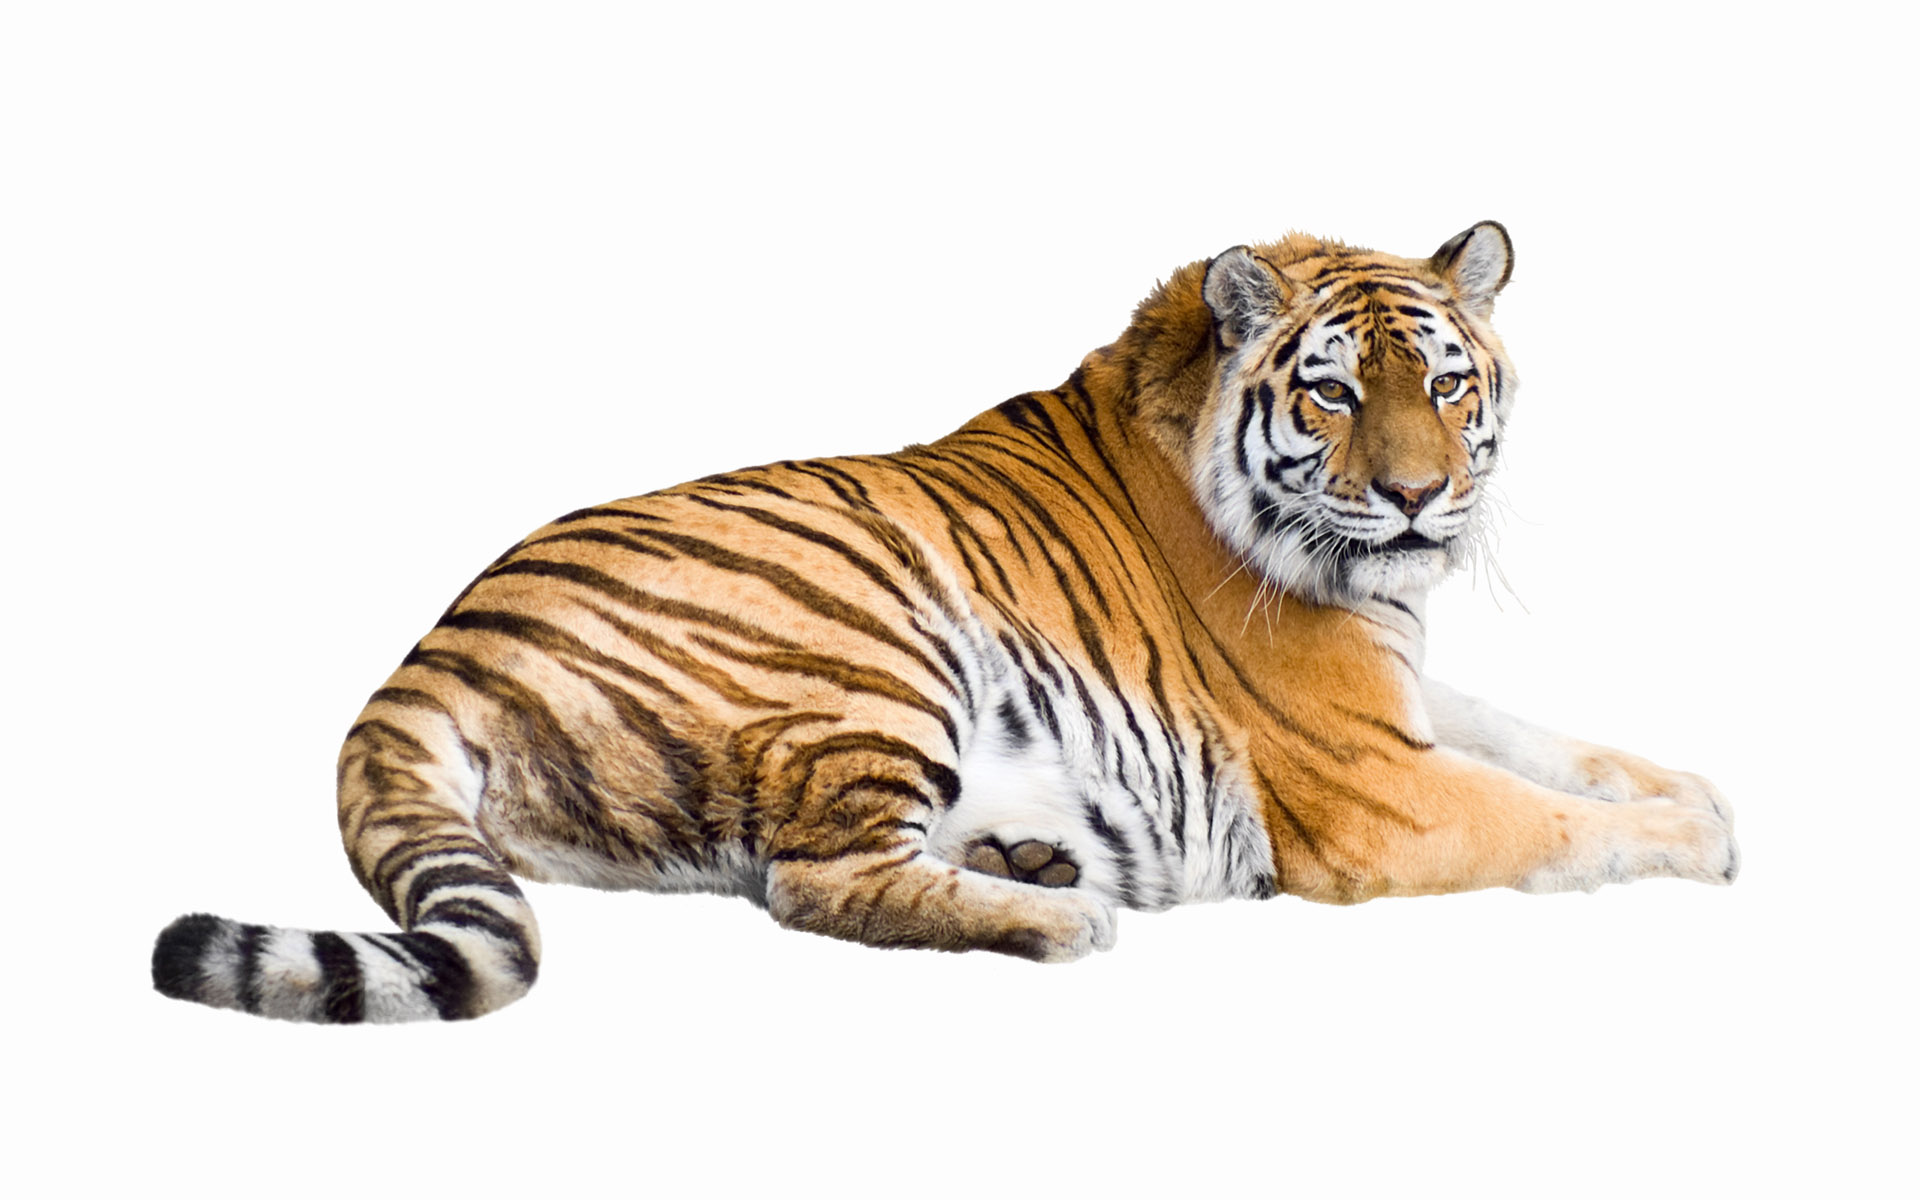
\includegraphics[scale=0.6]{/Users/alberto/Desktop/tiger.jpg}  %el parámetro scale permite agrandar o achicar la imagen. En el nombre de archivo puede especificar directorios
\label{kk1}
\caption{Tiger: Dificultad Difícil} 
\end{figure}

\newpage
\section{Valoración de los resultados obtenidos}

A continuación se muestran los resultados de la ejecución del algoritmo pasándole las distintas imágenes como entrada y seleccionando algunos puntos:

\begin{figure}[H] %con el [H] le obligamos a situar aquí la figura
\centering
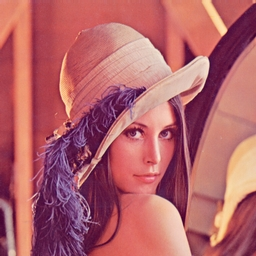
\includegraphics[scale=0.6]{/Users/alberto/Desktop/lena.png}  %el parámetro scale permite agrandar o achicar la imagen. En el nombre de archivo puede especificar directorios
\label{kk1}
\caption{Lena} 
\end{figure}

La imagen funciona bien si los puntos son relativamente cercanos, y como se observa sobre todo el contorno del sombrero es el que mejor se ajusta.

\begin{figure}[H] %con el [H] le obligamos a situar aquí la figura
\centering

\includegraphics[scale=0.6]{/Users/alberto/Desktop/black.png}  %el parámetro scale permite agrandar o achicar la imagen. En el nombre de archivo puede especificar directorios
\label{kk1}
\caption{Black} 
\end{figure}

\begin{figure}[H] %con el [H] le obligamos a situar aquí la figura
\centering

\includegraphics[scale=0.6]{/Users/alberto/Desktop/black_2.png}  %el parámetro scale permite agrandar o achicar la imagen. En el nombre de archivo puede especificar directorios
\label{kk1}
\caption{Black 2} 
\end{figure}

Si los puntos se seleccionan en las esquinas del rectángulo, o en línea recta se observa que se ajustan perfectamente. En cambio si el camino necesita hacer un giro se ajusta peor.

\begin{figure}[H] %con el [H] le obligamos a situar aquí la figura
\centering

\includegraphics[scale=0.6]{/Users/alberto/Desktop/circle_black.png}  %el parámetro scale permite agrandar o achicar la imagen. En el nombre de archivo puede especificar directorios
\label{kk1}
\caption{Circle black} 
\end{figure}

En este caso el ajuste es muy malo, se observa como la curva nunca se ajusta y son necesarios puntos bastante cercanos para que el ajuste sea relativamente aceptable.

\begin{figure}[H] %con el [H] le obligamos a situar aquí la figura
\centering
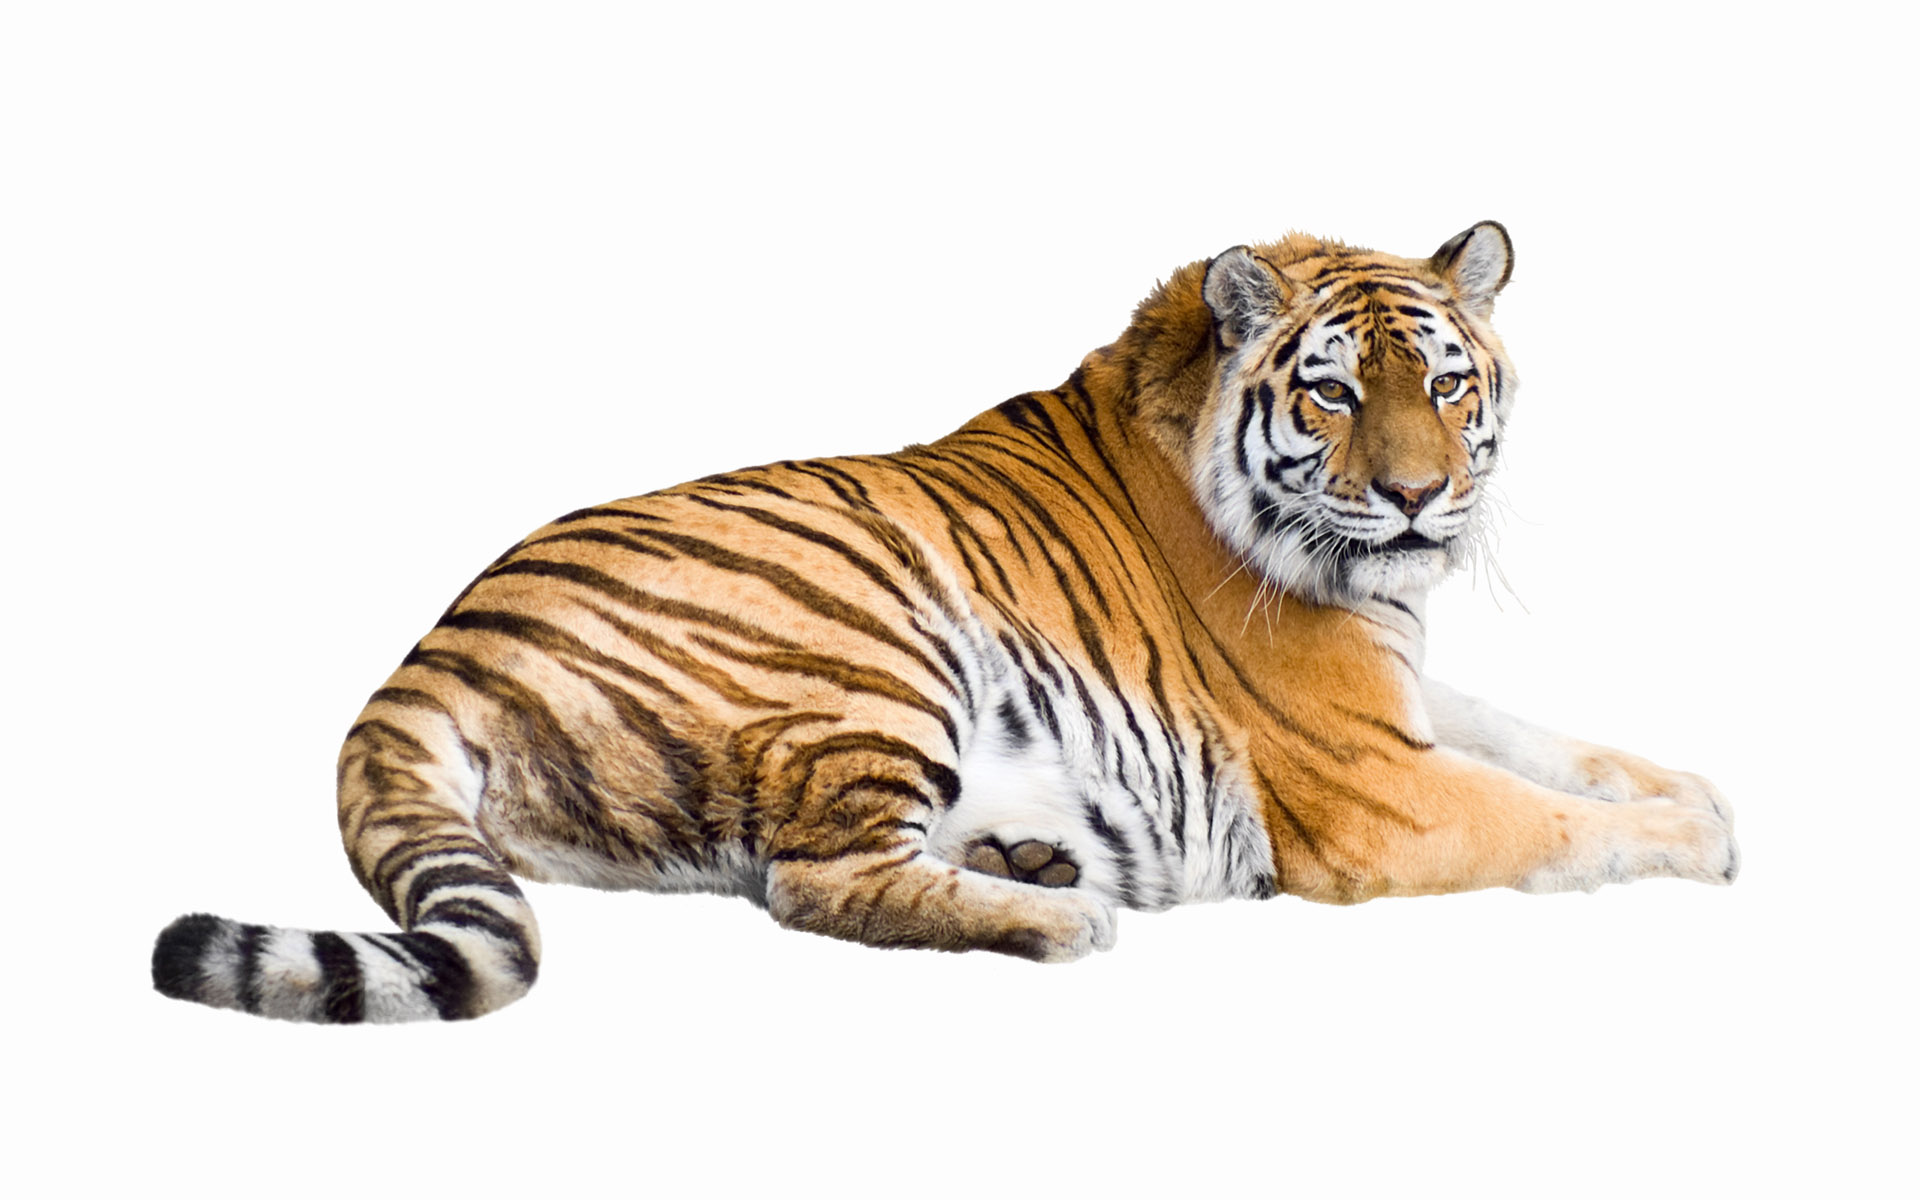
\includegraphics[scale=0.6]{/Users/alberto/Desktop/tiger.png}  %el parámetro scale permite agrandar o achicar la imagen. En el nombre de archivo puede especificar directorios
\label{kk1}
\caption{Tiger} 
\end{figure}

Ahora el ajuste del cuerpo se observa que es aceptable, aunque en la cara el ajuste es mucho mejor.



%------------------------------------------------


\end{document}